% sections/fingerprinting.tex
% 2. Website Fingerprinting on Tor

This section provides a background on The Onion Router (Tor) and the website fingerprinting attack which can neutralize the anonymity that Tor provides.

\subsection{Tor}

Tor is one of the most popular anonymizing networks, which distributes user's communications over several places on the Internet.
The distribution helps user's final destination not to be linked to a single point. Tor can be considered as an overlay network on top of the internet which directs TCP streams to different proxies.
In this network, packets take a random path through several relays, instead of taking a direct route.
These layers cover the user path such that it will not be possible to tell where the data comes from, or where it is going.
Such a pathway in Tor is called a private network pathway.
The Tor client application is responsible of creating this private pathway by incrementally building a circuit of encrypted connections.
The circuit is constructed hop by hop, which means each individual relay is only aware of the previous and next hop.
That is to say, individual relays never can identify the complete path. In order to build circuits, Tor makes use of authenticated DH key exchange encrypted with symmetric keys \cite{TorPage, dingledine2004tor}. Figure~\ref{fig:tor} demonstrates how Tor works.


\begin{figure}[h]
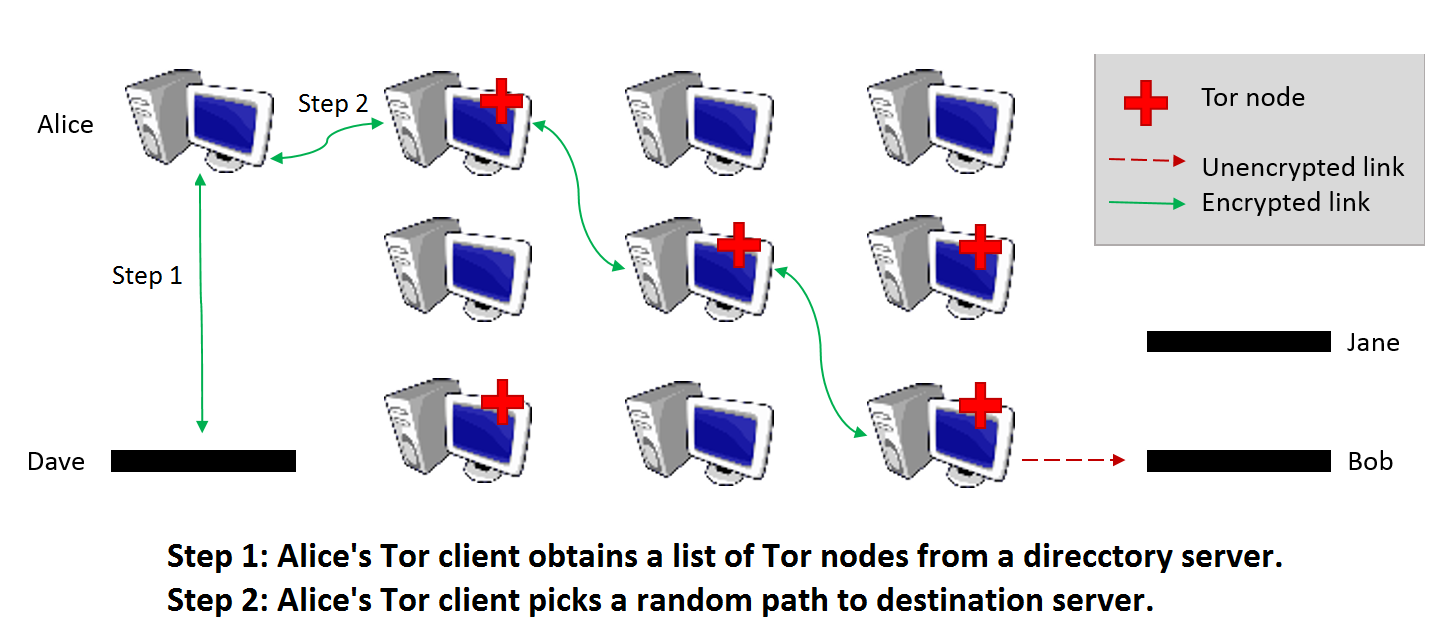
\includegraphics[width=1\columnwidth]{figures/tor.png}
\centering
\caption{The Onion Router (Tor)~\cite{TorPage}}
\label{fig:tor}
\end{figure}


The design described above aims to support a variety of anonymity goals. However, if an attacker can see both ends of the private pathway, Tor will fail.
For example, suppose the attacker watches the Tor relay to which the user enters the network, and also watches the website she visits; in this case, the attacker can correlate volume and timing information on the two sides.
To cope with this problem, Tor came up with the idea of {\it entry guards}, where each Tor client randomly selects a few relays as entry points for her first hop.
If those relays are not observed by an attacker, the user is secure.
But, needless to say, there is always a probability of losing anonymity~\cite{TorPage}.

\subsection{Website Fingerprinting}

Tor does not provide protection against all anonymity problems. In addition, the WF attack is still able to bypass its privacy mechanism. In the case of Tor, WF attack would take place between the user and the Guard node, or at the Guard node itself. In general, attack models can be divided into two categories: "closed world" and "open world" scenarios.  This section describes these attack models.

In the closed world model, the classifier can successfully recognize only web pages that it has already been trained on. Therefore, in this case, we deal with a small set of censored web pages. The open world scenario is when the adversary is capable of recognizing censored pages that might have not seen before \cite{TorBlog}.


Figure~\ref{fig:attack} illustrates the attack model of website fingerprinting. We also consider the WF adversary as local and passive, which means although the adversary is able to eavesdrop on user's traffic, he cannot modify it. It should be pointed out that the adversary will not be able to decrypt the traffic. Otherwise, he would not bother lunching a WF attack \cite{juarez14}.


\begin{figure}[h]

\includegraphics[width=0.7\columnwidth]{figures/attack_model.png}
\centering
\caption{Website Fingerprinting Attack Model~\cite{juarez14}}
\label{fig:attack}
\end{figure}


Juarez et al. in \cite{juarez14} divided the WF attack into two different types based on the number of the users it targets. In the first category, called \emph{targeted}, the adversary aims to obtain the browsing activity of a specific victim. In this case, since the adversary is able to train the classifier using the information of the victim, the attack is more successful. The adversary may even have enough information and background knowledge about the user and her behavior. So, it could be possible to guess and emulate the user configuration. Therefore, the accuracy of the classifier would increase. The second type of the attack is called \emph{non-targeted} or \emph{dragnet surveillance}, where a set of users, instead of one, are targeted by the attacker. In this case, ISP, entry guard, or Internet exchanges serves the attacker.  In other words, the attacker is able to intercept the traffic of many users by using such servers. A classifier in the non-targeted attack is trained based on a specific setting and used for all communications.


